\begin{appendices}
\section{Organigramma}
	\subsection{Redazione}
		\rowcolors{2}{lightRowColor}{darkRowColor}
		\begin{longtable}{
			>{\centering}p{0.25\textwidth}
			>{\centering}p{0.15\textwidth}
			>{\centering\arraybackslash}p{0.25\textwidth} }

			\coloredTableHead
			\textbf{\color{white}Nome} &
			\textbf{\color{white}Data} &
			\textbf{\color{white}Firma}
			\tabularnewline
			\endhead

			% Contenuto della tabella
			% Nome & Data & Firma\\
			\VB & 2020-04-08 & 
\includegraphics[width=0.2\textwidth]{./res/img/FirmeComponenti/firma_VB.jpg} \\
			\MP & 2020-03-29 & 
\includegraphics[width=0.2\textwidth]{./res/img/FirmeComponenti/firma_MP.jpg} \\

			\rowcolor{white}\caption {Redazione}	\\

		\end{longtable}

	\subsection{Approvazione}
		\rowcolors{2}{lightRowColor}{darkRowColor}
		\begin{longtable}{
			>{\centering}p{0.25\textwidth}
			>{\centering}p{0.15\textwidth}
			>{\centering\arraybackslash}p{0.25\textwidth} }

			\coloredTableHead
			\textbf{\color{white}Nome} &
			\textbf{\color{white}Data} &
			\textbf{\color{white}Firma}
			\tabularnewline
			\endhead

			% Contenuto della tabella
			% Nome & Data & Firma\\
			\TV & - & - \\
			\VB & 2020-04-11 & 
\includegraphics[width=0.2\textwidth]{./res/img/FirmeComponenti/firma_VB.jpg} \\

			\rowcolor{white}\caption {Approvazione} \\

		\end{longtable}
\newpage
	\subsection{Accettazione dei componenti}
		\rowcolors{2}{lightRowColor}{darkRowColor}
		\begin{longtable}{
			>{\centering}p{0.25\textwidth}
			>{\centering}p{0.15\textwidth}
			>{\centering\arraybackslash}p{0.25\textwidth} }

			\coloredTableHead
			\textbf{\color{white}Nome} &
			\textbf{\color{white}Data} &
			\textbf{\color{white}Firma}
			\tabularnewline
			\endhead

			% Contenuto della tabella
			% Nome & Data & Firma\\
			\VB & 2020-03-12 & 
\includegraphics[width=0.25\textwidth]{./res/img/FirmeComponenti/firma_VB.jpg} \\
			\NF & 2020-03-12 & 
\includegraphics[width=0.2\textwidth]{./res/img/FirmeComponenti/firma_NF.jpg} \\
			\EG & 2020-03-12 & 
\includegraphics[width=0.2\textwidth]{./res/img/FirmeComponenti/firma_EG.jpg} \\
			\FJ & 2020-03-12 & 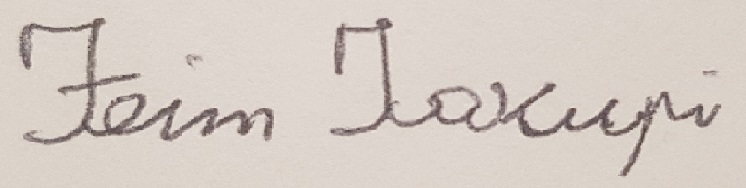
\includegraphics[width=0.2\textwidth]{./res/img/FirmeComponenti/firma_FJ.jpg} \\
			\MP & 2020-03-12 & 
\includegraphics[width=0.2\textwidth]{./res/img/FirmeComponenti/firma_MP.jpg} \\
			\LB & 2020-03-12 & 
\includegraphics[width=0.2\textwidth]{./res/img/FirmeComponenti/firma_LB.jpg} \\
			\AS & 2020-03-12 & 
\includegraphics[width=0.2\textwidth]{./res/img/FirmeComponenti/firma_AS.jpg} \\
			\AZ & 2020-03-12 & 
\includegraphics[width=0.2\textwidth]{./res/img/FirmeComponenti/firma_AZ.jpg} \\

			\rowcolor{white}\caption {Accettazione dei componenti} \\

		\end{longtable}

	\subsection{Componenti}
		\rowcolors{2}{lightRowColor}{darkRowColor}
		\begin{longtable}{
			>{\centering}p{0.25\textwidth}
			>{\centering}p{0.15\textwidth}
			>{\centering\arraybackslash}p{0.4\textwidth} }

			\coloredTableHead
			\textbf{\color{white}Nome} &
			\textbf{\color{white}Matricola} &
			\textbf{\color{white}Indirizzo email}
			\tabularnewline
			\endhead

			% Contenuto della tabella
			% Nome & Matricola & Indirizzo email\\
			\VB & 1143463 & veronica.barbieri.1@studenti.unipd.it \\
			\LB & 1122109 & luca.benetazzo@studenti.unipd.it \\
			\NF & 1143541 & nicoletta.fabro@studenti.unipd.it \\
			\EG & 1187021 & egon.galvani@studenti.unipd.it \\
			\FJ & 1163064 & feim.jakupi@studenti.unipd.it \\
			\MP & 1167693 & marco.positello@studenti.unipd.it \\
			\AS & 1144363 & alessandro.sgreva@studenti.unipd.it \\
			\AZ & 1171766 & antonio.zlatkovski@studenti.unipd.it \\

			\rowcolor{white}\caption {Componenti} \\

		\end{longtable}
\end{appendices}
